\begin{scanpage}{0154}{136}
\begin{center}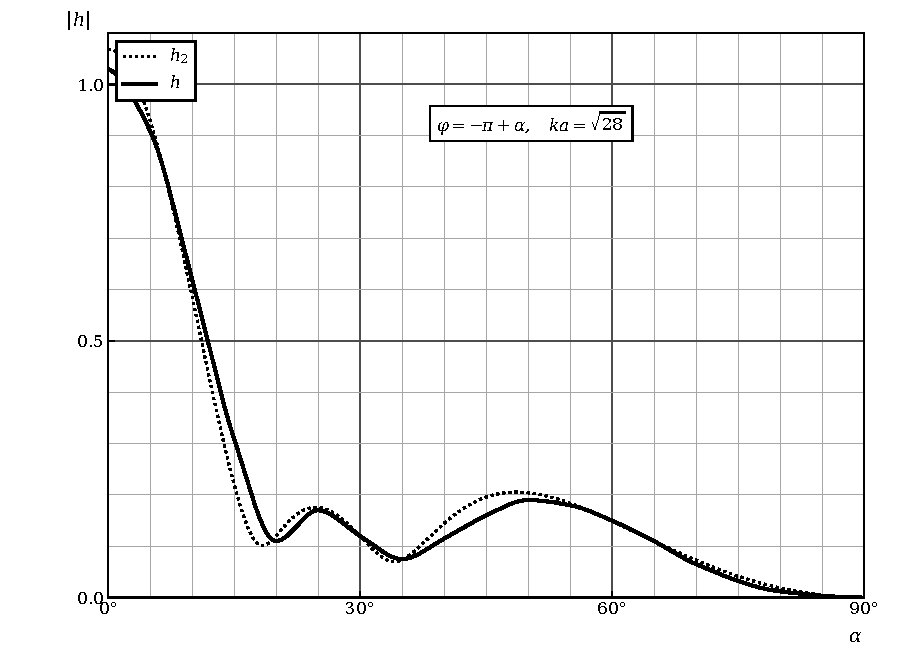
\includegraphics[width=.55\linewidth]{images/recreated/c-0154-fig51.pdf}\par
Figure 51. The same as Figure 49 when $\phi=-\pi+\alpha$.
\end{center}
strip ($\alpha=-\pi/2$), when the functions $e_0$ and $h_0$, and $e_1$ and $h_1$ lead to qualitatively incorrect results, the functions $e_2$ and $h_2$ give, as in the remaining cases, fully satisfactory results. Actually, the curve $|h_2|$ coincides almost everywhere with the curve $|h|$ (Figure 49--54) within the limits of graphical precision. But the calculated values of the function $|e_2|$ differ from the corresponding values of the function $|e|$ only by hundredths of a percent (Figure 55--62). The better agreement with the rigorous theory associated with the E-polarization is explained by the weaker interaction of the edges in this case. A certain discrepancy of the curves $|h_2|$ and $|h|$ in the vicinity of the principal scattering maximum is explained by the interpolation character of our equations.

As a consequence of the interpolation character of Equations (23.02), the integral scattering diameter obtained from Expressions (23.03) when $\alpha=0$ does not coincide with the integral diameter found by Clemmow [46] in the form of the first terms of an asymptotic expansion in inverse powers of $\sqrt{ka}$. However, our equations, as distinct from the similar equations obtained by other authors, allow one to calculate the scattering characteristics with any incident angles of the plane wave.
\end{scanpage}
